\chapter{Examples}
\label{chap:Examples}

The following examples are found in the {\tt Wave-DNA} source directory {\tt </path/to/wavedna/examples/>}. The case folder must contain the following files and directorie

\section{Default run}
\label{sec:Default run}

This example is found in {\tt examples/DefaultRun}.

If the {\tt run.DNA} options file is empty, the simulation is exclusively based on the default options. The result is a sinusoidal wave comprising ten emitted wave periods in a domain that comprises ten wavelengths. The is excited at the left (West) boundary and travels from left to right. The $\mathrm{CFL}$ number is equal to 0.1 and the spatial resolution is $N_{\mathrm{ppw}}=100$ points per wavelength. {\tt fields.dat} is the only output file as no probes are specified. The instantaneous obtained at a physical time of ten wave periods is shown in Fig.~\ref{fig:DefaultRun}. See Sec. \ref{sec:Default settings} and/or the source file {\tt src/io/iodefaultoptions.c} for the default settings.

\begin{figure}
    \centering
    {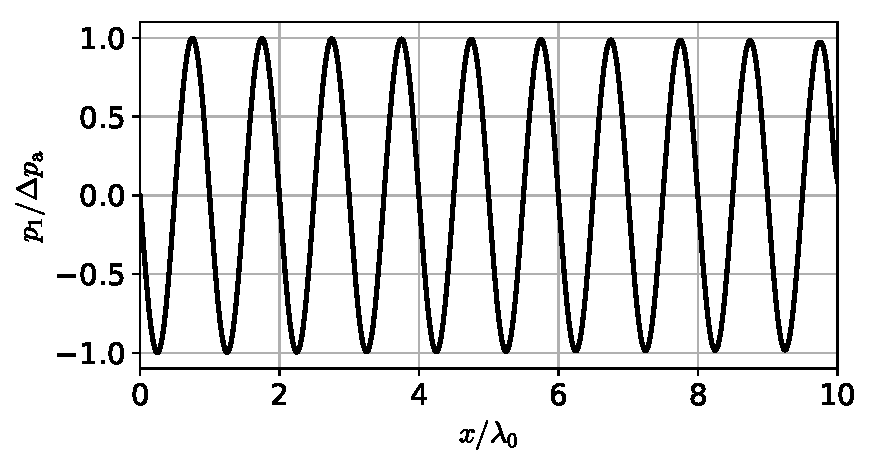
\includegraphics[width=0.5\textwidth]{DefaultRun.pdf}}
    \caption{\raggedright Instantaneous wave profile obtained for the default settings (empty {\tt run.DNA} file).}
    \label{fig:DefaultRun}
\end{figure}


\section{Absorbing vs reflecting boundary conditions}
\label{sec:Absorbing vs reflecting boundary conditions}

This example is found in {\tt examples/ScatteringAbsorbing}.

This test case illustrates the options for the boundary conditions. A Gaussian pulse is emitted as indicated by the red lines in Fig.~\ref{fig:BC} (see the {\tt run.DNA} file). The pulse is emitted at $x=0$ and travels from left to right. In Fig.~\ref{fig:BC} (a), the settings are:

{\tt
BoundaryConditionEast scattering\\
BoundaryConditionWest scattering
}

With the {\tt scattering} condition at the East boundary, the pulse is reflected at the boundary as indicated by the black line in Fig.~\ref{fig:BC} (a). In Fig.~\ref{fig:BC} (b), the settings are:

{\tt
BoundaryConditionEast absorbing\\
BoundaryConditionWest scattering
}

With the {\tt absorbing} condition at the East boundary, the pulse leaves the domain without reflection as shown by the black line in Fig.~\ref{fig:BC} (b). The settings for the West boundary are arbitrary as this boundary is the emission node in this case.

\begin{figure}
    \centering
    \subfloat[Scattering boundary]
    {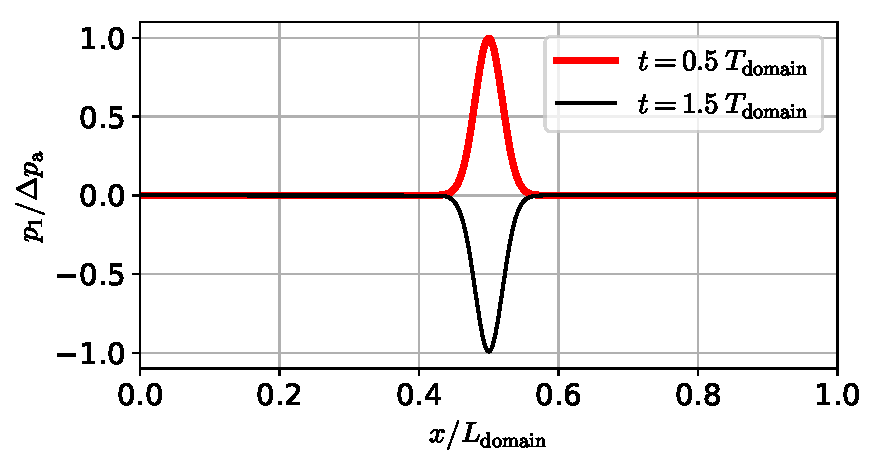
\includegraphics[width=0.49\textwidth]{px_scattering.pdf}} \
    \subfloat[Absorbing boundary]
    {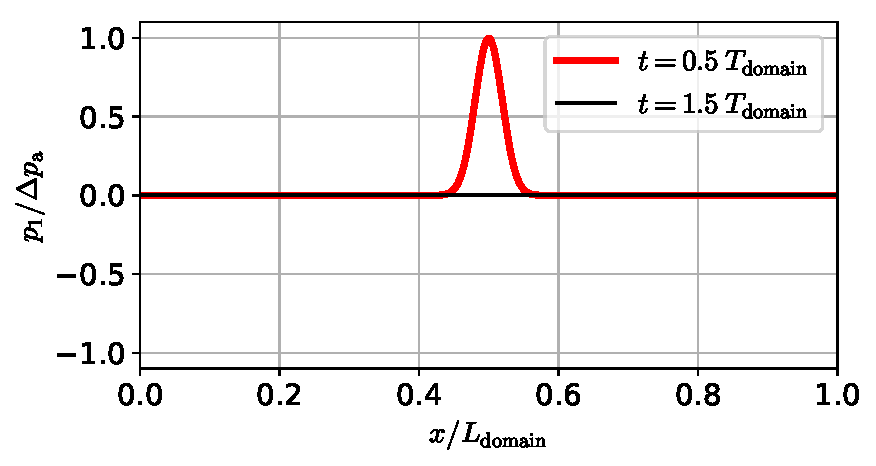
\includegraphics[width=0.49\textwidth]{px_absorbing.pdf}}
    \caption{\raggedright Illustration of the {\tt scattering} (b) and the {\tt absorbing} (b) boundary condition. A pulse travels from left to right (red lines). In (a), the pulse is reflected at the East domain boundary and travels back to the left (black line). In (b), the pulse passes the domain so that no reflection is visible (black line).}
    \label{fig:BC}
\end{figure}


\section{Shock-driven attenuation}
\label{sec:Shock-driven attenuation}

This example is found in {\tt examples/ShockDrivenAttenuation}.

This test case is concerned with the progressive deformation, shock formation, and shock-driven attenuation of an initially sinusoidal wave. The background medium is quiescent and the computational domain is at rest throughout the entire simulation. The $\mathrm{CFL}$ number is 0.05 with a spatial resolution of $N_{\mathrm{ppw}}=400$ points per wavelength $\lambda_0$ and a corrector weight of $\gamma=1.5$, set as follows:

{\tt
FluidNonLinearity 3.5
}

This rather high resolution is needed in order avoid excessive numerical dissipation due to the presence of the steep wavefront. The wave is emitted at the left boundary and travels to the right. The excitation amplitude and the nonlinearity coefficient $\beta$ are set in such a way that the nominal shock formation distance, given by \citep{Blackstock_1966}
\begin{equation}
    x_{\mathrm{sh}} = \dfrac{\rho_0 c_0^3}{2\pi \beta f_{\mathrm{a}}\Delta p_{\mathrm{a}}},
    \label{eq:xsh}
\end{equation}
takes the value $x_{\mathrm{sh}}=10$. At the shock formation distance, the progressively steepening wavefront first starts to develop a discontinuity. The red dashed line in Fig.~\ref{fig:shock_attenuation} represents the envelope $\widehat{p}_1$ owing to the Fay solution \citep{Fay_1931}, given by \citep{Blackstock_1966}
\begin{equation}
    \dfrac{\widehat{p}_1}{\Delta p_{\mathrm{a}}} = \dfrac{\pi}{1 + x/x_{\mathrm{sh}}}.
    \label{eq:Fay}
\end{equation}
The Fay solution is not applicable to the close vicinity of the emitter, but asymptotically approaches the wave profile decay at distances larger than approximately $3x_{\mathrm{sh}}$, where the initially sinusoidal has fully evolved into a saw-tooth shape. Fig.~\ref{fig:shock_attenuation} (a) shows that the wave profile exhibits only a minor decay prior to the shock formation distance, after which starts to approach the Fay envelope. Fig.~\ref{fig:shock_attenuation} (b) shows a detail of the fully developed saw-tooth pattern. It is noted that the predictor-corrector method drives the attenuation associated with the dissipation across the shock front. See \citet{Schenke_et_al_2022} for further discussions of this effect.

\begin{figure}
    \centering
    \subfloat[Decaying shock amplitude]
    {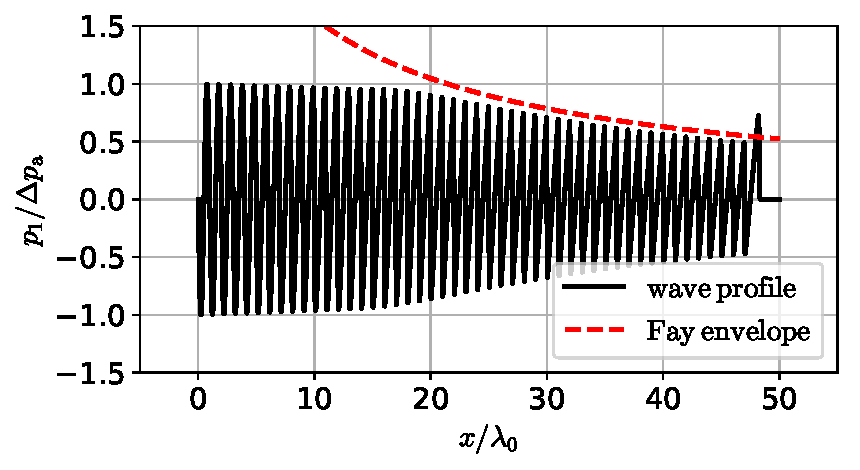
\includegraphics[width=0.49\textwidth]{shock_attenuation.pdf}}
    \subfloat[Detail of the saw-tooth profile]
    {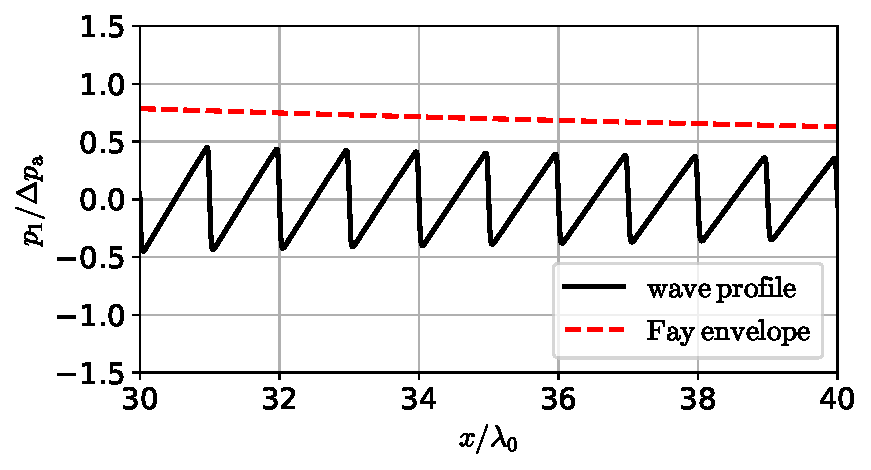
\includegraphics[width=0.49\textwidth]{shock_attenuation_detail.pdf}}
    \caption{\raggedright Initially sinusoidal and progressively steepening and shock-forming wave. As the wave has traveled past the shock formation distance $x_{\mathrm{sh}}=10\lambda_0$ (see Eq. \eqref{eq:xsh}) in subfigure (a), its amplitude starts to decay rapidly, asymptotically approaching the envelope of Fay solution \citep{Fay_1931} as given by Eq. \eqref{eq:Fay} \citep{Blackstock_1966}. Subfigure (b) depicts a detail of the fully developed saw-tooth profile.}
    \label{fig:shock_attenuation}
\end{figure}


\section{Moving emitter, boundary and flow}
\label{sec:Moving emitter, boundary and flow}

The following examples are found in {\tt examples/MovingBoundary}.

\subsection{Moving emitter}
\label{sec:Moving emitter}

This example is found in {\tt examples/MovingBoundary/RelativeEmitterMotion}.

This example illustrates how the Doppler shift due to the motion of an emitter relative to a quiescent medium can be reproduced with {\tt Wave-DNA}. A sine wave is excitated at the left (West) domain boundary and travels from left to right. The background flow field is quiescent:

{\tt BackgroundMotionMode quiescent}

The speed of sound is:

{\tt SoundSpeed 1500.0}

The moving boundary moves at a constant velocity magnitude of $500\:\mathrm{m/s}=c_0/3$, where the setting

    {\tt BoundaryMotionType linear}

is used to indicate a constant velocity of the boundary. The excitation location at the left boundary (default) is specified by:

{\tt ExcitationNode 0}

The initial position of the moving boundary is $x=0$ (default) and the fixed boundary is located at $x=0.18\:\mathrm{m}$ (12 times the unmodulted waveength $\lambda_0$), specified as follows:

{\tt
InitialMovingBoundaryPosition 0.0 \\
FixedBoundaryPosition 0.18
}

Hence, the moving boundary acts as a wave emitting boundary so that the acoustic wave is Doppler-shifted upon emission. In Fig.~\ref{fig:RelativeEmitterMotion} (a), the wave emitting boundary moves from right to left, hence against the direction of wave propagation, by setting:

{\tt MovingBoundaryVelocityAmplitude -500}

This causes a red-shift (frequency decrease) of the emitted wave. In Fig.~\ref{fig:RelativeEmitterMotion} (b), the wave emitting boundary moves from left to right, hence in the direction of wave propagation, by setting:

{\tt MovingBoundaryVelocityAmplitude 500}

This causes a blue-shift (frequency increase) of the emitted wave.

\begin{figure}
    \centering
    \subfloat[Red-shifted wave]
    {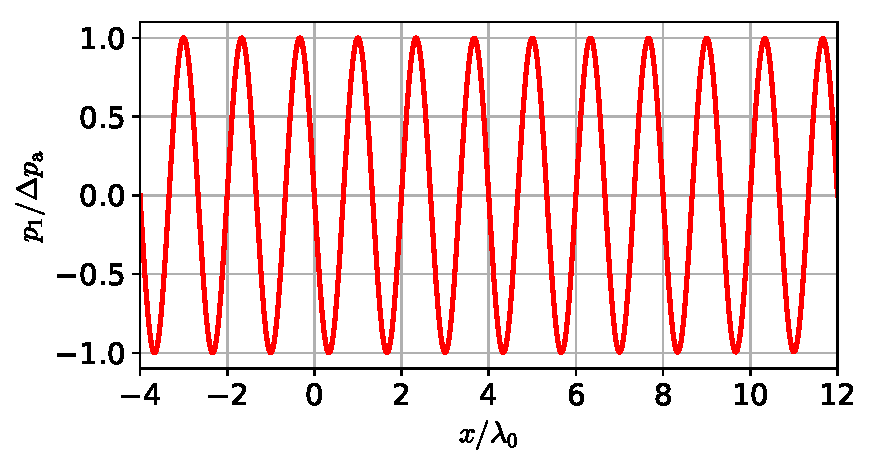
\includegraphics[width=0.49\textwidth]{Doppler_red.pdf}}
    \subfloat[Blue-shifted wave]
    {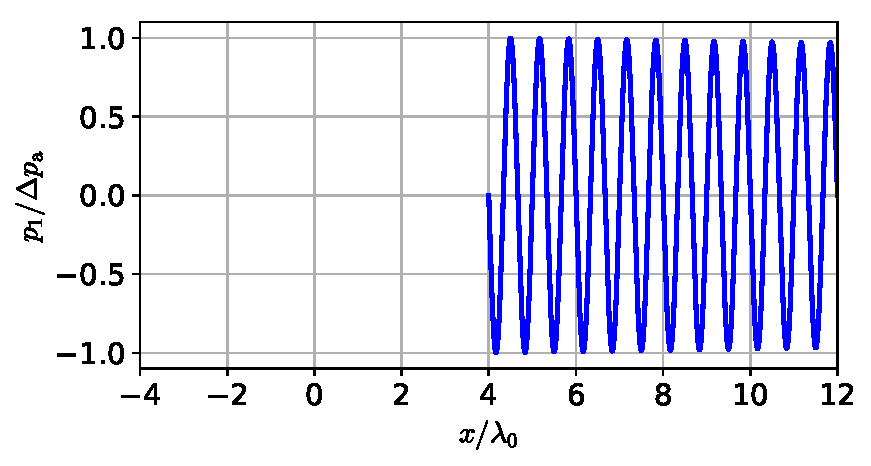
\includegraphics[width=0.49\textwidth]{Doppler_blue.pdf}}
    \caption{\raggedright Doppler-shift induced by an emitter moving relative to a quiescent medium: the wave is excited at the moving boundary. The wave emitting boundary starts at $x=0$ and moves in negative $x$-direction in (a), thereby red-shifting the emitted wave, and in positive $x$-direction in (b), thereby blue-shifting the emitted wave. The magnitude of the boundary velocity is $c_0/3$.}
    \label{fig:RelativeEmitterMotion}
\end{figure}


\subsection{Induced flow field}
\label{sec:Induced flow field}

This example is found in {\tt examples/MovingBoundary/InducedFlow}.

Fig.~\ref{fig:ConvectedWave} shows how an acoustic wave is Doppler-shifted by a temporaily constant and spatially uniform background flow field in one-dimensional Cartesian coordinates. In both Figs. \ref{fig:ConvectedWave} (a) and (b), the left domain boundary moves to the right with a velocity of $c_0/3$, and in both cases it induces a background flow field of the same velocity and direction by setting:

{\tt
BackgroundMotionMode coupledToMovingBoundary
}

In Fig.~\ref{fig:ConvectedWave} (a), the wave is excited at the moving boundary, which is initially at $x=0$ by setting:

{\tt
ExcitationNode 0
}

As a result, the wave travels from left to right and there is no relative motion between the wave emitter and the background flow field and the emitted wavelength $\lambda_0$ is not modulated. The instantaneous wave profile in Fig.~\ref{fig:ConvectedWave} is shown at two time instances in order to illustrate the variable position of the wave emitting boundary. In Fig.~\ref{fig:ConvectedWave} (b), the wave is excited at the fixed right boundary by setting:

{\tt
ExcitationNode 4800
}

Hence, the wave travels from right to left and the fixed wave emitting boundary is in relative motion to the encountered background flow field. This causes a blue-shift of the emitted wavelength.

\begin{figure}
    \centering
    \subfloat[Flow inducing and wave emitting boundary]
    {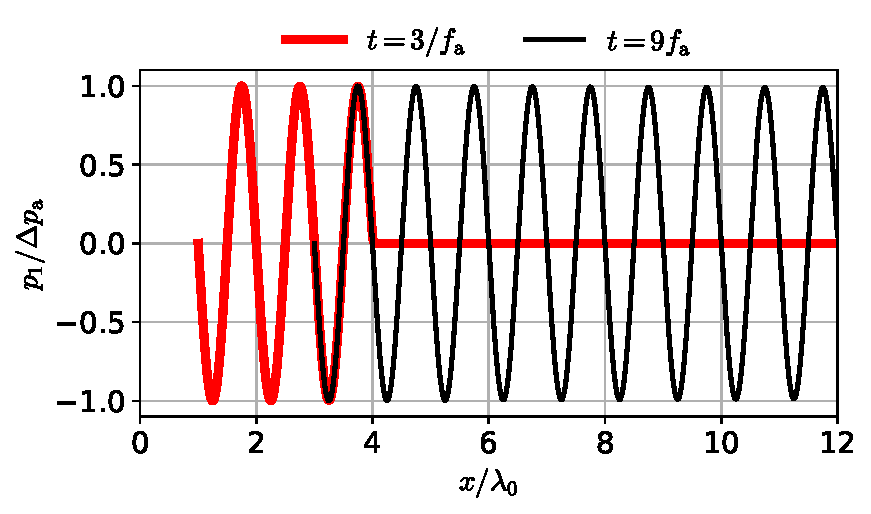
\includegraphics[width=0.49\textwidth]{InducedFlow.pdf}}
    \subfloat[Flow moving relative to fixed emitter]
    {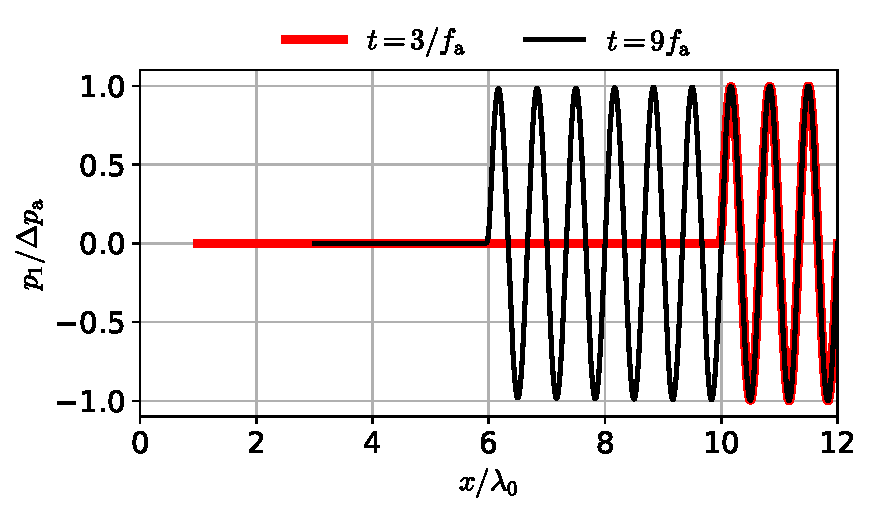
\includegraphics[width=0.49\textwidth]{RelativeEmitterMotion.pdf}}
    \caption{\raggedright Illustration of a flow-induced Doppler shift. The left domain boundary is initially at $x=0$ and moves from left to right with a velocity of $c_0/3$. At the same time, the moving boundary induces a temporarily and spatially constant background flow field. In (a), the wave is excited at the moving boundary and travels from left to right. As there is no relative motion between background medium in (a), the emitted wavelength is not modulated. In (b), the wave is excited at the right boundary and travels from right to left, so that the wave emitting boundary is in relative motion to the encountered background flow. This causes a blue-shift of the emitted wave.}
    \label{fig:ConvectedWave}
\end{figure}


\section{Possible combinations of moving boundaries, flow fields and emitters}
\label{sec:Possible combinations of moving boundaries, flow fields and emitters}

In {\tt examples/MovingBoundary/PossibleCombinations}, the possible combinations of setting up moving boundaries wave-emitting or non-emitting boundaries and quiescent or induced moving flow fields are demonstrated. Table \ref{tab:hierarchyMotion} illustrates the hierarchy of possible configurations.

The initial positions of the moving and the fixed boundary determines, which of them is identified as the West and the East boundary, where the boundary further to the left is the West boundary. The boundary condition (either {\tt scattering} or {\tt absorbing}) is assigned to the West and East boundaries, respectively ({\tt BoundaryConditionWest} or {\tt BoundaryConditionEast}). Irrespective of which of the two domain boundaries is the moving one, any of the two boundaries can be the wave-emitting boundary. It is recalled from Sec. \ref{sec:Wave excitation} that the wave-emitting boundary with instantaneous position $R\left(t\right)$ is alawys associated with grid node $0$, whereas the fixed boundary with position $R_{\mathrm{stat}}$ is always associated with grid node $N_{\mathrm{points}}-1$. Finally, for each of the four configurations of moving vs fixed and emitting vs non-emitting boundaries, the moving boundary can be a flow inducing one or move relative to a quiescent background flow field. This gives the eight different configurations as listed in Table \ref{tab:hierarchyMotion}.

Each of the test cases in this example directory is set up in such a way that waves move past the domain domain boundary. Hence, the test cases also illustrate how the wave-absorbing boundary condition is applied in these configurations.


\begin{table}[htb]
    \centering
    \begin{tabular}{|l|l|l|}
        \hline
        \multirow{4}{*}{Moving West boundary} & \multirow{2}{*}{Emitting West boundary ({\tt ExcitationNode} 0)}                       & Quiescent flow \\
        \cline{3-3}
                                              &                                                                                        & Induced flow   \\
        \cline{2-3}
                                              & \multirow{2}{*}{Emitting East boundary ({\tt ExcitationNode} $N_{\mathrm{points}}-1$)} & Quiescent flow \\
        \cline{3-3}
                                              &                                                                                        & Induced flow   \\
        \cline{1-3}
        \multirow{4}{*}{Moving East boundary} & \multirow{2}{*}{Emitting West boundary ({\tt ExcitationNode} $N_{\mathrm{points}}-1$)} & Quiescent flow \\
        \cline{3-3}
                                              &                                                                                        & Induced flow   \\
        \cline{2-3}
                                              & \multirow{2}{*}{Emitting East boundary ({\tt ExcitationNode} $0$)}                     & Quiescent flow \\
        \cline{3-3}
                                              &                                                                                        & Induced flow   \\
        \hline
    \end{tabular}
    \caption{Eight possible configurations of moving vs fixed, emitting vs non-emitting, and flow inducing vs relatively moving (quiescent flow) boundaries.}
    \label{tab:hierarchyMotion}
\end{table}


\section{Slowly oscillating emitter and flow field}
\label{sec:Slowly oscillating emitter and flow field}


The example of a slowly oscillating emitter is concerned with a slowly oscillating domain boundary, where ``slow'' means that the frequency $f_{\mathrm{b}}$ of the sinusoidal motion of the domain boundary is smaller than the emitted wave frequency $f_{\mathrm{a}}$. In this example, a spherically symmetric wave is considered, where the settings for the background flow field are:

{\tt
Geometry 3dSphericallySymmetric \\
BackgroundMotionMode quiescent \\
BackgroundVelocityScalingFactor 2.0
}

for a quiescent background medium to which the wave-emitting boundary is in relative motion or

    {\tt
        BackgroundMotionMode coupledToMovingBoundary\\
    }

for the case where the moving boundary displaces the fluid. The settings for the oscillatory boundary motion are:

{\tt
BoundaryMotionType oscillating \\
BoundaryMotionStartTime 0.0e-0 \\
BoundaryMotionEndTime 2.3e10 \\
InitialMovingBoundaryPosition 0.015 \\
FixedBoundaryPosition 0.195 \\
MovingBoundaryVelocityAmplitude 375 \\
MovingBoundaryFrequency 1e4
}

Hence, the boundary oscillates around an initial radius of $R_0=0.015\:\mathrm{m}$, which corresponds to one wavelength with an emitted wave frequency of $f_{\mathrm{a}}=100\:\mathrm{kHz}$ (ten times larger than the frequency the boundary motion) and a speed of sound of $c_0=1500\:\mathrm{m/s}$. With a velocity amplitude of $375\:\mathrm{m/s}$ of the boundary motion, the maximum Mach number is 0.25.

For reference, Fig.~\ref{fig:pr_oscilattingEmitter_staticBoundary} shows the instantaneous wave profile for a resting wave-emitting boundary ({\tt MovingBoundaryVelocityAmplitude 0}), where the wave decays like $1/r$ as indicated by the red dashed line. Figs. \ref{fig:rt_oscillatingEmitter} (a), (b), and (c) show the space-time diagrams for the resting, the relatively moving, and the flow-inducing moving boundaries, respectively. In the latter case, the characteristics posses a slight curvature due the variable background flow field in which the acoustic wave propagates.

\begin{figure}
    \centering
    {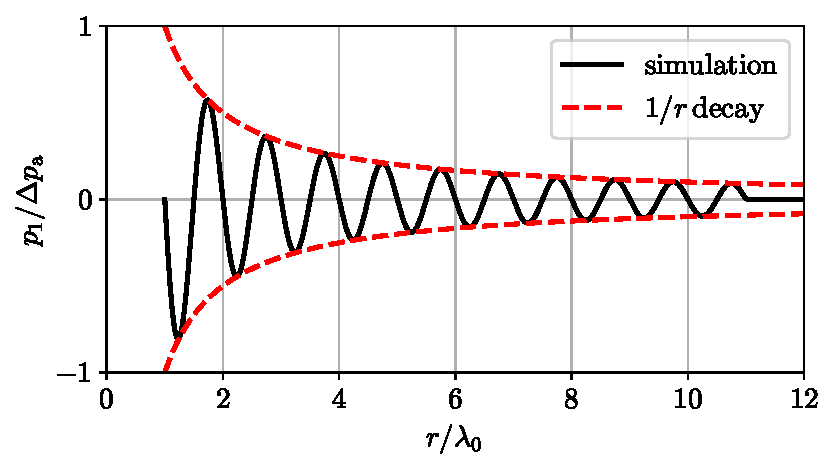
\includegraphics[width=0.5\textwidth]{pr_oscilattingEmitter_staticBoundary.pdf}}
    \caption{\raggedright spherically symmetric wave decaying like $1/r$.}
    \label{fig:pr_oscilattingEmitter_staticBoundary}
\end{figure}

\begin{figure*}
    %\baselineskip=12pt
    \subfloat[Fixed wave-emitting boundary]
    {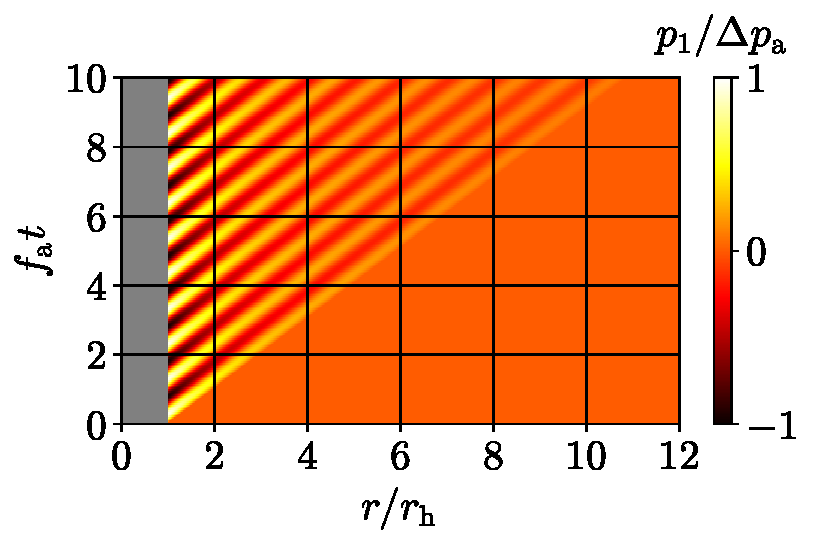
\includegraphics[width=0.33\textwidth]{rt_oscilattingEmitter_staticBoundary.pdf}}
    \subfloat[Oscillating wave-emitting boundary in a quiescent medium]
    {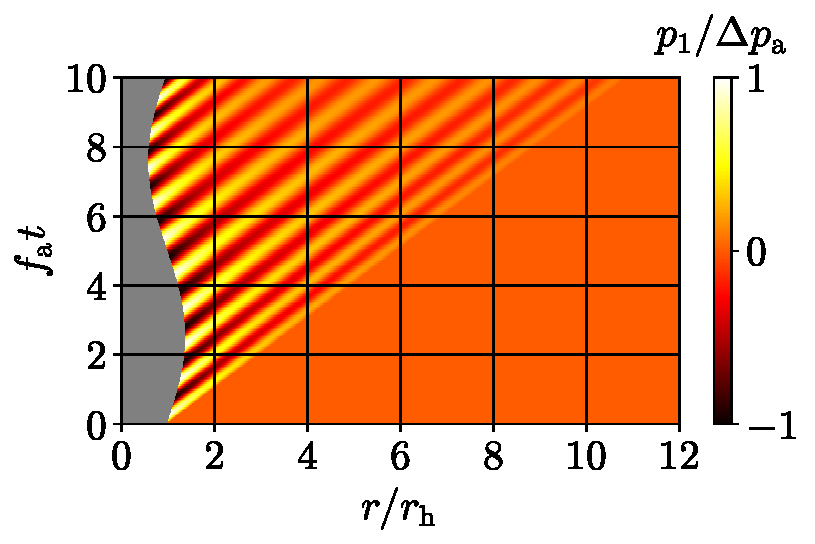
\includegraphics[width=0.33\textwidth]{rt_oscilattingEmitter_quiescent.pdf}}
    \subfloat[Oscillating flow-inducing wave-emitting boundary]
    {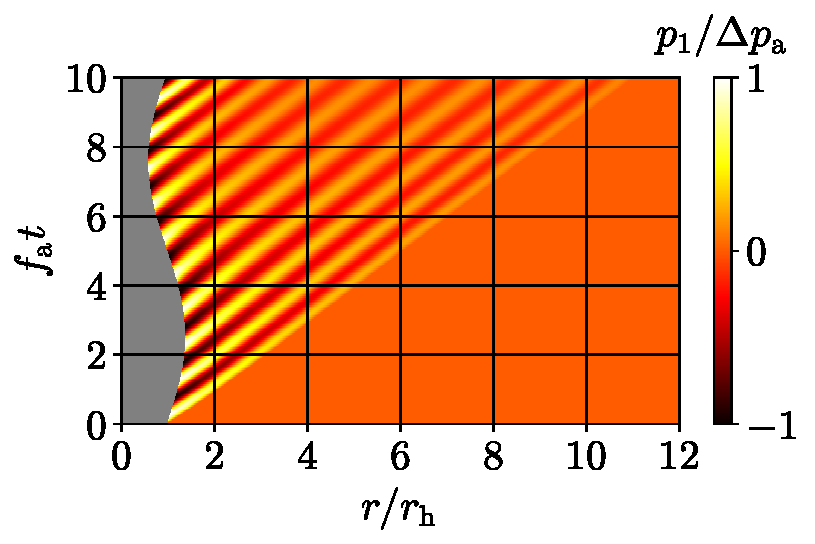
\includegraphics[width=0.33\textwidth]{rt_oscilattingEmitter_inducedFlow.pdf}}
    \caption{\raggedright Space-time diagrams of an oscillating wave-emitting boundary, where ten acoustic wave periods are emitted during one oscillation cycle of the moving boundary.}
    \label{fig:rt_oscillatingEmitter}
    %\vskip1in
\end{figure*}


\section{Acoustic black and white holes}
\label{sec:Acoustic black and white holes}

The following examples show how {\tt Wave-DNA} can be used to simulate the acoustic wave propgation in acoustic black and white hole configurations \citep{Schenke_et_al_2022_PoF}. The individual test case folders, containing illustrative acoustic black and white hole examples, include python postprocessing scripts in order to produce space-time diagrams, the plots of the instantaneous wave profiles, and the acoustic pressure evolution at the sonic horizon.

It is important to note that rather than representing compressible background flow fields with variable $\rho_0$ and $c_0$, the acoustic black/white hole configurations are model systems for acoustic waves propagating in accelerating flow fields of any (also subsonic) velocity magnitude. The reason for the acoustic black/white hole being such a convenient system for the computational study of acoustic waves in accelerating flow fields lies in the fact that they allow to trap a wave characteristic at the point of sonic transition, the sonic horizon, where it is subject to both a constant background flow velocity and a constant background flow acceleration. Due to the non-zero acceleration, the neighbouring characteristics are either converging towards or diverging away from the sonic horizon.

In the acoustic black hole example shown here, nonlinearities are neglected ($\beta=0$ and $\mathcal{L}=0$). Fig.~\ref{fig:BH} exemplarily shows (a) the space-time diagram and (b) the instantaneous acoustic pressure profiles for an acoustic black hole. The entire physical domain in Fig.~\ref{fig:BH} is initially located outside the acoustic black hole. Subsequently, the moving wave emitting boundary collapses and eventually passes the sonic horizon while emitting outgoing characteristics. The example in Fig.~\ref{fig:BH} is realized by the following boundary settings:

{\tt
BoundaryMotionType stationaryBlackHole \\
InitialMovingBoundaryPosition 1.60175 \\
FixedBoundaryPosition 1.75175
}

The stationary sonic horizon radius and the geometry settings are:

{\tt
Geometry 3dSphericallySymmetric \\
BackgroundMotionMode coupledToMovingBoundary \\
HorizonRadius 1.5
}

With these settings, the wave emitting boundary radiates a wavetrain that propagates in positive $r$-direction. At the same time, the spherical moving boundary collapses and induces an inward-directed spherically symmetric background fluid flow that satisfies Eq. \eqref{eq:u0_spherical}. The boundary satisfies Eq. \eqref{eq:R} so that a stationary flow field is obtained. The data at the stationary sonic horizon is written to the output file {\tt horizon.dat}. This file can be consulted to examine the evolution of the acoustic pressure and the acoustic (velocity) potential at the sonic horizon.

Fig.~\ref{fig:WH} exemplarily shows (a) the space-time diagram and (b) the instantaneous acoustic pressure profiles for an acoustic white hole, which can be seen as the inverse problem of the acoustic black hole. This time, the entire physical domain is initially located inside the acoustic white hole. Subsequently, the wave emitting boundary expands and eventually passes the sonic horizon while emitting ingoing characteristics. The sonic horizon radius, the speed of sound, and the emitted wave frequency are the same as in Fig.~\ref{fig:BH}. The settings to trap the same emitted wave period at the sonic horizon as in the acoustic black hole configuration are as follows:

{\tt
BOUNDARYMOTION \\
BoundaryMotionType stationaryWhiteHole \\
InitialMovingBoundaryPosition 1.3824 \\
FixedBoundaryPosition 1.2359
}

Furthermore, Fig.~\ref{fig:WH} shows the results for the nonlinear wave, which exhibits the well-known nonlinear wave-steepening. The settings to achieve the nonlinear wave propagation behavior, in this particular case dominated by the constitutive nonlinearity represented by the nonlinearity coefficient $\beta$ ({\tt FluidNonLinearity}), are:

    {\tt
        FluidNonLinearity 3.5 \\
        LocalNonlinearity True
    }

In the acoustic white hole in Fig.~\ref{fig:WH}, the characteristics converge towards the sonic horizon so that the acoustic wave is progressively blue-shifted while the acoustic wave amplitude increases over time.

\begin{figure*}
    %\baselineskip=12pt
    \subfloat[Space-time diagram]
    {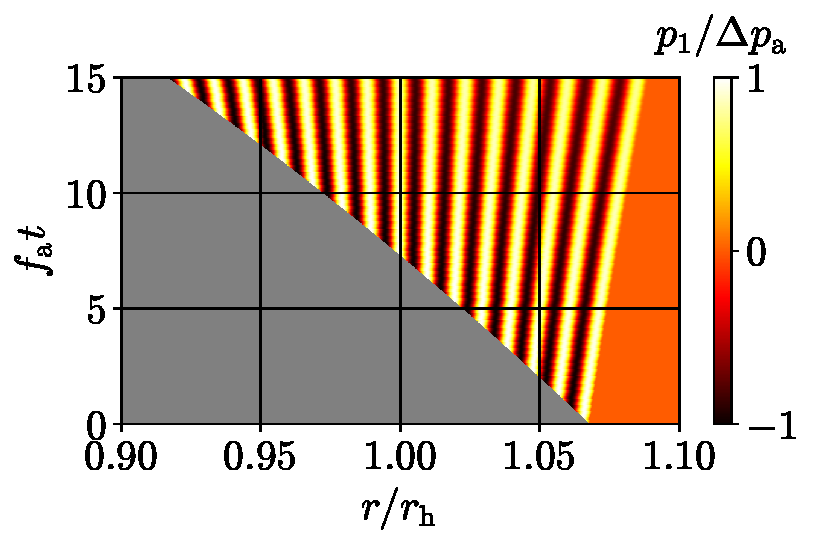
\includegraphics[width=0.45\textwidth]{rt_smallABH.pdf}}
    \subfloat[Instantaneous acoustic pressure profile]
    {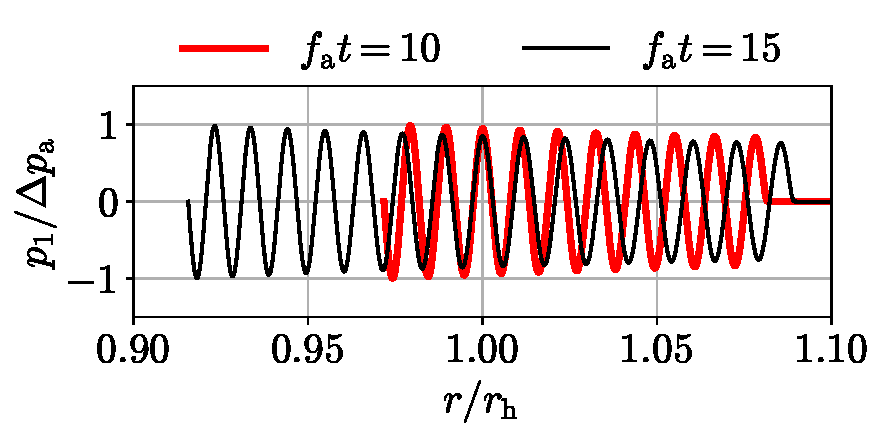
\includegraphics[width=0.45\textwidth]{pr_smallABH.pdf}}
    \caption{Example of an acoustic black hole.}
    \label{fig:BH}
    %\vskip1in
\end{figure*}


\begin{figure*}
    %\baselineskip=12pt
    \subfloat[Space-time diagram]
    {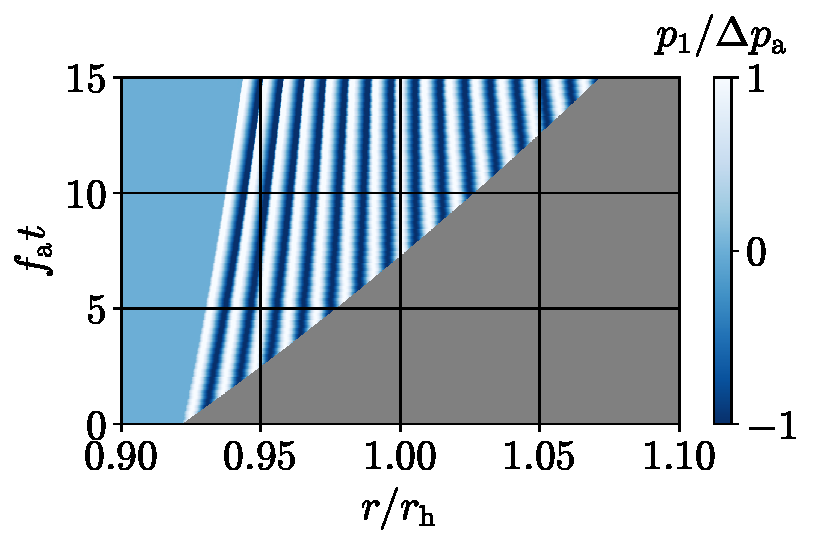
\includegraphics[width=0.45\textwidth]{rt_smallAWH_nonlin.pdf}}
    \subfloat[Instantaneous acoustic pressure profile]
    {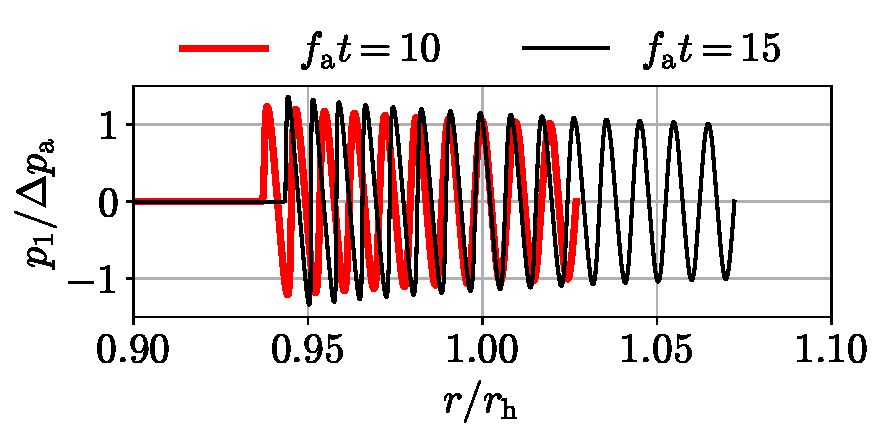
\includegraphics[width=0.45\textwidth]{pr_smallAWH_nonlin.pdf}}
    \caption{Example of an acoustic white hole.}
    \label{fig:WH}
    %\vskip1in
\end{figure*}



